\documentclass[smaller,aspectratio=169]{beamer}
% \usepackage{beamerthemesplit}
\setbeamersize{text margin left=0.2em}  % <- like this
\setbeamersize{text margin right=0.1em} % <- like this

\addtobeamertemplate{navigation symbols}{}{ \hspace{1em}    \usebeamerfont{footline}%
\insertframenumber / \inserttotalframenumber }

\usetheme{Marburg}

\usepackage[utf8]{inputenc}
\usepackage[T1]{fontenc}
\usepackage[francais]{babel}
\usepackage{graphicx}

\author{Md Tahsir Ahmed Munna}
\title{PhD Enrolling Interview}
%\subtitle{}
%\logo{}
\institute{Skoltech}
\date{25 May 2020}
%\subject{}
%\setbeamercovered{transparent}
%\setbeamertemplate{navigation symbols}{}

\begin{document}
	\maketitle
	\begin{frame}
		\frametitle{Outline}
		\tableofcontents{}
	\end{frame}
	
	\section{Achievements}
	
	\begin{frame}
		\frametitle{Achievements}
		\begin{center}
			\begin{itemize}
				\item Finalist of the Ilya Segalovich Yandex Scientific Award 2019, Russia.
				\item Fellowship 2018-2020, Bangabandhu Science and Technology Fellowship Trust, Bangladesh.
				\item Winner, National App Hackathon 2016, Bangladesh
				\item News: Nominated for HSE’s Silver Nestling Award in 2019.
				
			\end{itemize}
			 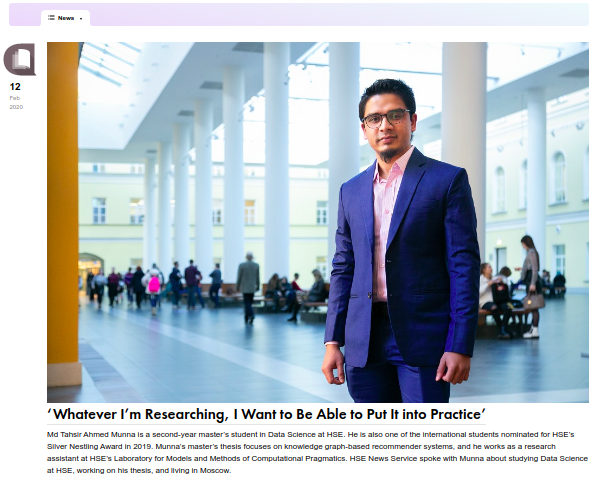
\includegraphics[width=5cm]{img/prospective student.png}
		\end{center}
		
	\end{frame}
	
	
	\section{Past and Recent Work}
	
	\subsection{Dissertation and Project Work}
	\begin{frame}
	\frametitle{Past and Recent Work}
	\textbf{Master of Science Thesis}
		\begin{itemize}
			\item COVID19 patients contact tracing and Cross-domain Co-Author Recommendation based on Knowledge Graph Embedding
		\end{itemize}
		\textbf{Project Work}
		\begin{itemize}
			\item User Intent Prediction by Factorization Machines (FM) Model.
			\begin{itemize}
			    \item Project from "Huawei"
			    \item Lead by "Skoltech"
			\end{itemize}
		\end{itemize}
	\textbf{Lab Work}
	\begin{itemize}
	    \item Research Intern: Laboratory for Models and Methods of Computational Pragmatics (HSE)
	    \begin{itemize}
	        \item Supervised by Dmitry I. Ignatov
	        \item Team: Recommender System
	    \end{itemize}
	\end{itemize}
	\end{frame}
	
	\begin{frame}{Master Thesis Discussion}
	\begin{center}
	     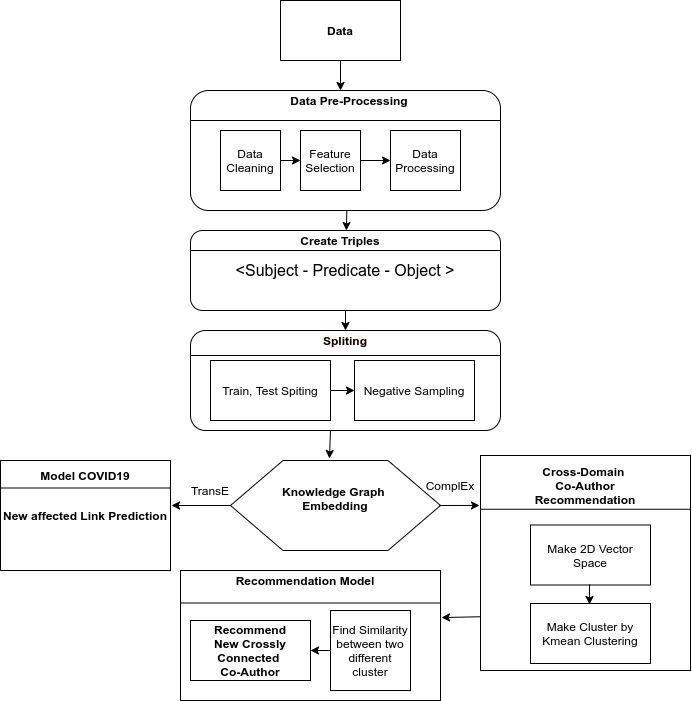
\includegraphics[width=7cm]{img/KG_RecSys.png}
	\end{center}
	   
	\end{frame}
	
	\begin{frame}{Project Work}
In my study I rely on the second-order factorization machines (FM). The case for regression-like FM model is shown below. 	
$$\hat y(\mathbf x)=w_0+\sum_{i=1}^n w_i x_i + \sum_{i=1}^{n-1}\sum_{j=i+1}^{n} \langle \mathbf v_i, \mathbf v_j \rangle x_i x_j, \mbox{ where }$$

\noindent $w_0 \in \mathbb R$ is the model intercept, $w_i \in \mathbb R$ is the coefficient for attribute $x_i \in \mathbb R$ of an input vector $\mathbf{x}$ with $n$ attributes and vectors $\mathbf v_i, \mathbf v_j \in \mathbb{R}^k$ form a dot product estimate $\langle \mathbf v_i, \mathbf v_j \rangle$  for the second order coefficient of the pairwise interaction of attributes $x_i$ and $x_j$.
	    
	\end{frame}
	
	
	\subsection{Research Work}
	\begin{frame} %Bilan
		\frametitle{Past and Recent Work}
	
	
	\begin{columns}[T] % align columns
    \begin{column}{.40\textwidth}
    %\color{blue}\rule{\linewidth}{2pt}
    \textbf{Research Work}
    \begin{itemize}
	    \item Nine Published Article
	    \item Seven are in Scopus indexed
	    \item Two are Open access Journal papers
	    \item Submit abstract of my thesis paper at RecSys 2020
	\end{itemize}
    \end{column}%
    \hfill%
    \begin{column}{.60\textwidth}
    %\color{blue}\rule{\linewidth}{2pt}
    \textbf{Google Scholar Profile}
    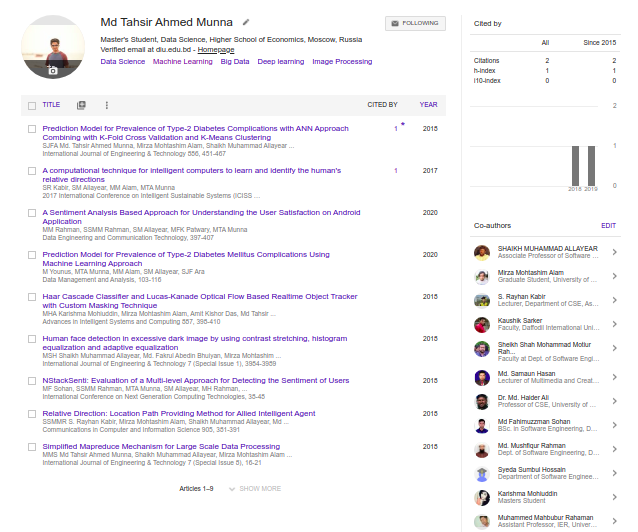
\includegraphics[width=8cm]{img/paper.png}
    \end{column}%
    \end{columns}
	\end{frame}
	

	\section{Why I choose this program?}
	\begin{frame} 
		\frametitle{Why I choose this program?}
		\begin{itemize}
			\item My Master Program is "Data Science" Which is directly match with my PhD program.
			\item My previous research field is also related to my PhD program.
			\item Now, Data Science is the most potential area for future career.
		\end{itemize}
	\end{frame}
	
	\section{Why Skoltech?}
	\begin{frame}{Why Skoltech?}
	\begin{itemize}
	    \item Research potentiality and funding
	    \item My current research area and my prospective professor lab (Natural Language Processing) work have a good match.
	    \item I have passed two years at Moscow and fall in love with this culture.
	\end{itemize}
	    
	\end{frame}
	
	\section{Why you choose me?}
	\begin{frame}{Why you choose me?}
	\begin{itemize}
	    \item Have research and programming skills.
	    \item Hard Worker and Have patient.
	    \item Can run after the Dream.
	\end{itemize}
	    
	\end{frame}
	
	\section{Research Interest}
	\begin{frame}{Research Interest}
	\textbf {User Profiling in Recommendation Systems}
	\begin{itemize}
	    \item Knowledge Graph
	    \begin{itemize}
	        \item Entity profiling in knowledge graphs
	    \end{itemize}
	    \item Deep Learning
	    \begin{itemize}
	        \item  Multi-Channel Deep Fusion Approach
	    \end{itemize}
	  \item Ready to accept professor suggestion on my field 
	\end{itemize}
	    
	\end{frame}
	\section{End}
	\begin{frame}
	    \begin{center}
	       % \textbf{Thank You}\\
	       % \textbf{Happy to Hear your Questions :)}
	       
\includegraphics[width=8cm]{img/questions.png}
	    \end{center}
	   %\rule{\linewidth}{.01pt}
	   \flushleft \small{Md Tahsir Ahmed Munna\footnote{ makhmedmunna@edu.hse.ru | ORCID ID: 0000-0001-9269-502X | Scopus ID: 57202903135}}
	\end{frame}
    
  
	
\end{document}